\documentclass[12pt]{book}
\usepackage{tgschola}
\usepackage[margin=1in]{geometry}
\usepackage{tikz}
\usetikzlibrary{shapes.geometric, arrows, positioning}

\title{The Hibike and Runtime Guide}
\date{\today}
\author{The Hibike Team}
\begin{document}
\maketitle

\tableofcontents

\chapter{Introduction}
The driving principle behind PiE is running a robotics competition. This means many things:
logistics, provinding mentorship and guidance, organizing events,
providing an interface for programming the robot, and making
the robot work. Keep in mind that this guide addresses only one aspect
of the competition; plumbing is not everything. With that said, it is still a good
idea to have a plumber on hand when pipes start to leak.
\section{A Brief Overview of the Control Stack}
For our purposes, there are four elements involved in controlling the robot.
\begin{enumerate}
	\item Dawn: the main interface that students use. Takes inputs from the controller,
	and shows data and errors to students.
	\item Runtime: the program in charge of monitoring and communication. Sends and receives data from
	Dawn, as well as monitoring Hibike and StateManager.
	\item StateManager: a data store. Provides a central place to store and retrive data from Hibike
	and Runtime.
	\item Hibike: the program that communicates with sensors. Handles low-level protocol details.
\end{enumerate}
\section{An Analogy}
A simple way to explain the role of each component in the stack, from Dawn to Hibike, is
as an analogy to a company.

Dawn is the CEO, the main person in charge. Every other system starts or stops
on her word, and follows her orders to the letter. Runtime is the middle manager. He
passes information from underlings on to the boss, relays her orders to them, and makes
sure that they are working. StateManager is the record-keeper. He stores information
that Hibike and Runtime give him, and retrieves it when they ask for it. Hibike is
in charge of a bunch of interns, the sensors. She asks them to periodically give her
updates on what they are doing, and fires them if they don't.
\section{A Diagram of the Stack}
\begin{center}
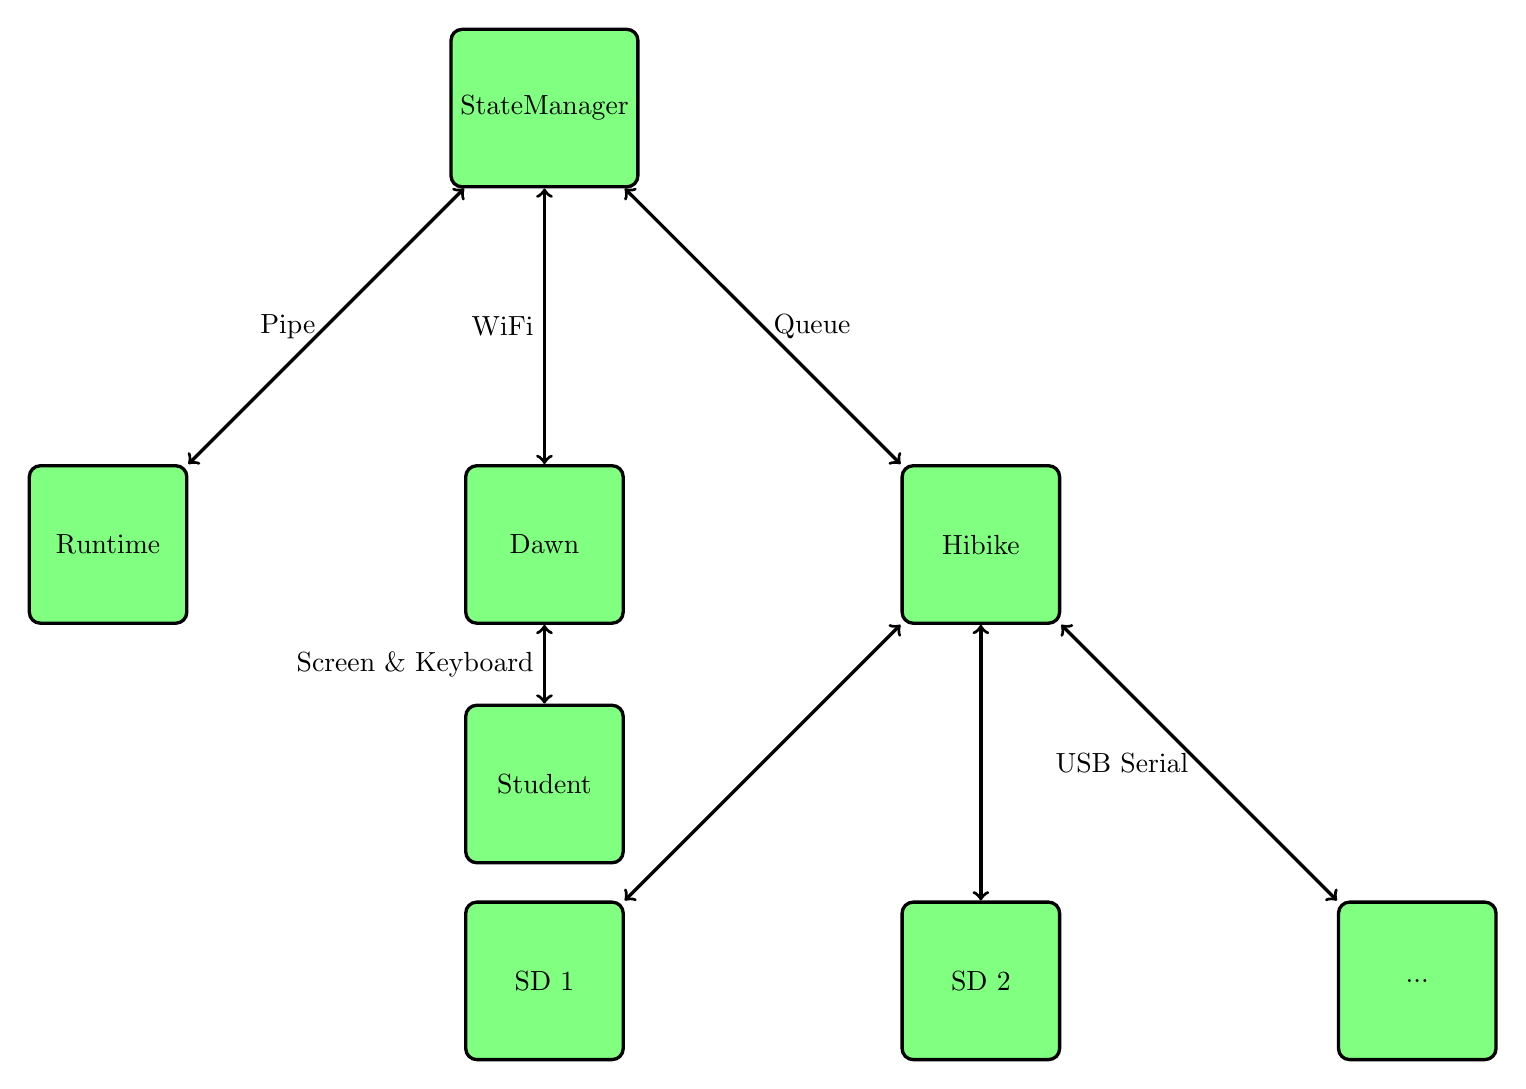
\begin{tikzpicture}[node distance=3.5cm, part/.style={
        rectangle,
        rounded corners,
        draw=black,
        text=black,
        fill=green!50,
        minimum size=2cm,
        very thick
    }, label/.style={
        rectangle,
        rounded corners,
        draw=black,
        very thick
    }, arrow/.style={
        very thick, <->, =>stealth
    }]
    \node (smgr) [part] {StateManager};
    \node (dawn) [part, below=of smgr] {Dawn};
    \node (student) [part, below=of dawn, yshift=2.5cm] {Student} ;
    \node (runtime) [part, left=of dawn] {Runtime};
    \node (hibike) [part, right=of dawn] {Hibike};
    \node (smrt1) [part, below=of hibike] {SD 2};
    \node (smrt2) [part, right=of smrt1] {...};
    \node (smrtmore) [part, left=of smrt1] {SD 1};
    \draw [arrow] (student) -- node[anchor=east] {Screen \& Keyboard} (dawn);
    \draw [arrow] (smgr) -- node[anchor=east] {Pipe} (runtime);
    \draw [arrow] (smgr) -- node[anchor=east] {WiFi} (dawn);
    \draw [arrow] (smgr) -- node[anchor=west] {Queue} (hibike);
    \draw [arrow] (hibike) -- (smrt1);
    \draw [arrow] (hibike) -- node[anchor=east] {USB Serial} (smrt2);
    \draw [arrow] (hibike) -- (smrtmore);

\end{tikzpicture}
\end{center}
\chapter{Hibike}
Hibike is in charge of low-level sensor communication, and all the gory
details that are involved. It is divided into two modules:
\begin{itemize}
	\item \texttt{hibike\_message.py}

	The low-level details of the
	Hibike communications protocol. Handles things like encoding into packets and checksums.
	\item \texttt{hibike\_process.py}

	The ``supervisor'' of sensors.
	Communicates with sensors, sends data to runtime, and reacts to orders from StateManager.
\end{itemize}

Alongside these main modules, there are various testing modules:
\begin{itemize}
	\item \texttt{virtual\_device.py}

	Virtual devices, for testing Hibike's read and write capabilities.
	\item \texttt{hibike\_tester.py}

	A test module that wraps a Hibike process with a nicer interface.
\end{itemize}

\section{Design Choices and Explanations}
Hibike is packet-based and works over USB, specifically serial.

\paragraph{Why USB?}

In previous years, a custom communications protocol was used, over custom cables.
This provided the advantage of real-time and configurability; however, debugging was very difficult,
and developing for smart sensors more so. The Beaglebone doesn't provide real-time guarantees
anyways, and USB provides cheap, commodity cables and well-tested software.

\paragraph{Why packets?}

Most protocols are packet-based, and serial is not a packet-based communications link.
Packets make it easy to tell when data begins and ends.

\paragraph{Why serial?}

Arduino provides a well-tested serial library, so communication with any Arduino is easy
over serial. In addition, implementing and using serial is relatively simple compared
to many other types of USB connection, such as HID (used by keyboards and mice). Some
flexibility and speed is lost as a result of this abstraction, but much more is gained
in ease of use.

\section{The Hibike Protocol}
\subsection{A Quick Introduction}
We make a few starting assumptions concerning the endpoints of communication: the device controlling a sensor is a Smart Device (SD), and a Beaglebone Black (BBB) is used as the central control board of each robot and thus is in charge of communicating with each Smart Device. These two communicate with each other via serial: the Beaglebone running pySerial and the Smart Device by using the built-in serial library. As each Smart Device communicates with the Beaglebone on its own separate port, we conveniently have no need to worry about any race conditions or other problems arising from concurrency.

Hibike abstracts every Smart Device as a set of (parameter, value) pairs.
The hibike protocol supports three ways of interacting with these parameters:
\begin{itemize}
\item Subscribing to regular updates of specific paramters
\item Polling specific parameters
\item Writing to specific parameters
\end{itemize}

Refer to Section 7 for an outline of the general behavior of the Hibike protocol.

\subsection{Message Format}

All messages have the relatively simple structure of Message ID, Payload, and Checksum as
depicted below. A more complete description of each field is given below the diagram.

\begin{center}
	\begin{tabular}{|c|c|c|c|}
	\hline
	Message ID & Payload Length & Payload & Checksum \\
	(8 Bits) & (8 Bits) & (Length Varies) & (8 Bits) \\
	\hline
	\end{tabular}
\end{center}

\begin{itemize}
	\item Message ID
	\begin{itemize}
		\item An 8-bit ID specifying the type of message.
		\item More information about this field in the following sections.
	\end{itemize}
	\item Payload Length
	\begin{itemize}
		\item An 8-bit unsigned integer, specifying the number of bytes in the payload.
	\end{itemize}
	\item Payload
	\begin{itemize}
		\item Varies depending on the type of message sent.
	\end{itemize}
	\item Checksum
	\begin{itemize}
		\item An 8-bit checksum placed at the end of every message.]
		\item The current scheme XORs every other byte in the message.
	\end{itemize}
\end{itemize}

\subsection{UID Format}
Each smart device is assigned an 88-bit UID with the following fields.

\begin{center}
	\begin{tabular}{|c|c|c|}
	\hline
	Device Type & Year & ID \\
	(16 Bits) & (8 Bits) & (64 bits) \\
	\hline
	\end{tabular}
\end{center}

\begin{itemize}
	\item Device Type
	\begin{itemize}
		\item 16-bit ID specifying the Type of a Smart Device
		\item Device types are enumerated in Section 5
	\end{itemize}
	\item Year
	\begin{itemize}
		\item 8-bit ID corresponding to the competition year that the Smart Device was manufactured for.
		\item The 2015-2016 season will correspond to 0x00
	\end{itemize}
	\item ID
  	\begin{itemize}
  		\item Randomly generated 64-bit number that will uniquely identify each Smart Device within a specific device type and year.
  		\item With 64-bit IDs, the probability of a hash collision with 1000 of 1 type of device per year is roughly 0.05\%
	\end{itemize}
\end{itemize}

\subsection{Parameters and Bitmaps}

\begin{itemize}
	\item Hibike abstracts every smart device as a set of parameters that map to values
	\item Each smart device contains some number of paramaters, which can be read/written to.
	\item Parameters can have many types. The following types are supported:
	\begin{itemize}
		\item \texttt{bool}
		\item \texttt{uint8\_t}
		\item \texttt{int8\_t}
		\item \texttt{uint16\_t}
		\item \texttt{int16\_t}
		\item \texttt{uint32\_t}
		\item \texttt{int32\_t}
		\item \texttt{uint64\_t}
		\item \texttt{int64\_t}
		\item \texttt{float}
		\item \texttt{double}
	\end{itemize} CAUTION: Arduino's doubles are only 4 bytes long (same as a float), so an
	Arduino's Double is the same as python's Float. Do not use this type
	unless your arduino is actually cranking out 8 bytes.
	\item Some paramaters are read only, some are write only, and some support both.
	\item A config file will describe the paramaters for each Device Type (name, type, permissions).
	\item Some packets encode sets of parameters in the form of bitmaps.
	\begin{center}
		\begin{tabular}{|c|c |c| c|}
		\hline
		Params & Value 0 & \ldots & Value 15 \\
		(16 bits) & (Optional and Variable) & \ldots & (Optional and Variable) \\
		\hline
		\end{tabular}
	\end{center}
	\begin{itemize}
		\item Params - 16-bit bitmap describing a set of parameters. The nth bit of
		Params, where the LSB is the 0th bit, references the nth paramater of
  		a device.
		\item Value{[}0-15{]} - DeviceWrite and DeviceData send actual values for
  		each param in Params. The value field for param n will only be present
  		if bit n in Params is set. The size and type of each value field
  		depends on param number and device type, and is described in a config
  		file.
  	\end{itemize}
\end{itemize}

\subsection{Enumerations}
\begin{center}
    \begin{tabular}{|c|c|}
        \hline
        ID & Message Type \\
        \hline
        0x10 & Ping \\
        0x11 & Subscription Request \\
        0x12 & Subscription Response \\
        0x13 & Device Read \\
        0x14 & Device Write \\
        0x15 & Device Data \\
        0x16 & Device Disable \\
        0x17 & Heartbeat Request \\
        0x18 & Heartbeat Response \\
        0xFF & Error \\
        \hline
    \end{tabular}
\end{center}

\subsection{Message Descriptions}
\begin{enumerate}
    \item Ping: BBB pings SD for enumeration purposes.
        The SD will respond with a SubscriptionResponse packet.
        
        Payload format:
        \begin{center}
            \begin{tabular}{|c|c|}
                \hline
                Empty \\
                (0 bits) \\
                \hline
            \end{tabular}
        \end{center}
        Direction: BBB $\Rightarrow$ SD

    \item SubscriptionRequest: BBB requests data to be returned at a given interval.
        \begin{itemize}
            \item Params is a bitmap of paramaters being subscribed to.
            \item The SD will respond with a Sub Response packet with a delay and
                bitmap of params it will acutally send values for, which may not be
                what was requested, due to nonexistent and write-only parameters.
            \item If too many parameters are subscribed to, the Smart Device may have
                to send multiple DeviceData packets at each interval.
            \item A delay of 0 indicates that the BBB does not want to receive data.
            \item Non-zero delay with 0 Params will still subscribe to empty
                updates!!!
        \end{itemize}
        Payload format:
        \begin{center}
            \begin{tabular}{|c|c|}
                \hline
                Params & Delay \\
                (16 bits) & (16 bits) \\
                \hline
            \end{tabular}
        \end{center}
        Direction: BBB $\Rightarrow$ SD
    \item SubscriptionResponse: SD sends (essentially) an ACK packet with its UID,
        params subscribed to, and delay.

        Payload format:
        \begin{center}
            \begin{tabular}{|c|c|c|}
                \hline
                Params & Delay & UID \\
                (16 bits) & (16 bits) & (88 bits) \\
                \hline
            \end{tabular}
        \end{center}
        Direction: BBB $\Leftarrow$ SD
    \item Device Read: BBB requests some values from the SD.
        \begin{itemize}
            \item The SD should respond with DeviceData packets with values for all
                the readable params that were requested.
            \item If all the values cannot fit in one packet, multiple will be sent.
        \end{itemize}

        Payload format:
        \begin{center}
            \begin{tabular}{|c|}
                \hline
                Params \\
                (16 bits) \\
                \hline
            \end{tabular}
        \end{center}
        Direction: BBB $\Rightarrow$ SD


\end{enumerate}

\section{The Hibike Process}
\texttt{hibike\_process.py} handles communication with sensors and StateManager.
Initialization and running happen in this series of steps:
\begin{enumerate}
    \item Hibike asks the operating system for a list of serial ports that match
        those used by Arduinos.
    \item It verifies that these ports are working, and opens them for communication.
    \item Hibike checks that each port contains a smart sensor by pinging it.
    \item Each device is given a reading thread, a writing thread, and a write queue.
    \item Alongside the device threads, a read batching thread and a cleanup
        thread are started. The batch thread sends all reads to StateManager
        at certain intervals. The cleanup thread removes disconnected devices.
    \item Hibike tells all devices to stop sending data. Once the devices
        respond, StateManager subscribes to each device for each of
        its parameters.
    \item Afterwards, Hibike receives and reacts to commands from StateManager.
\end{enumerate}

\subsection{An Explanation of the Architecture}
Each part of the structure of the Hibike process has its place, and has
been designed in deliberately. Here are explanations for certain parts.

\paragraph{Reader and Writer Threads}
Reading from a serial connection using nonblocking communication means that it
is easily possible to receive an incomplete packet even if the communications
link is reliable; thus, we use blocking reads. We don't want to stop reading
from every other sensor if one is taking a while, so we use threads to
periodically switch between sensors.

\paragraph{The Write Queue}
If a device sends a heartbeat request, we want to respond quickly
without going all the way to StateManager. Thus, we have a write queue, allowing
both the main thread and the read thread to write packets.

\paragraph{The Batch Thread}
Inter-thread communication is quick, but inter-process communication is slow.
Consequentially,
Hibike threads can quickly talk to each other, but talking to StateManager, which
runs in a separate process, is quite time-consuming. Instead of
sending any device data as soon as it is read, it is easier to bundle many
reads up and send them all at once. The batch thread is responsible for this.

\paragraph{The Cleanup Thread}
When a device disconnects, its resources remain in use. The read
and write threads sit idle, and the serial port remains open. This
can cause problems if a new device appears on an existing serial port,
so it is useful to clean up the resources. At the same time, it
can take up to 30 seconds to close a serial port, which is unacceptably
long for Hibike to wait. Therefore, a separate thread is put in charge
of such things.

\section{Testing}
\chapter{StateManager}
\chapter{Runtime}
\end{document}
